Via het Software\index{Software}\index{Desktop!Software} icoon, zie figuur \ref{fig:de_software_icon}, op de dash\index{Dash!Software} kan je de applicatie opstarten om de software op je systeem te beheren.

\begin{figure}[H]
\includegraphics{software-dash.png}
	\caption{Software icoon}
	\label{fig:de_software_icon}
\end{figure}

Je kan er applicaties mee toevoegen aan je systeem, verwijderen van je systeem of de bestaande applicaties updaten naar de laatste versie. Met een dubbel klik op het icoon start je de Software applicatie op.

\begin{figure}[H]
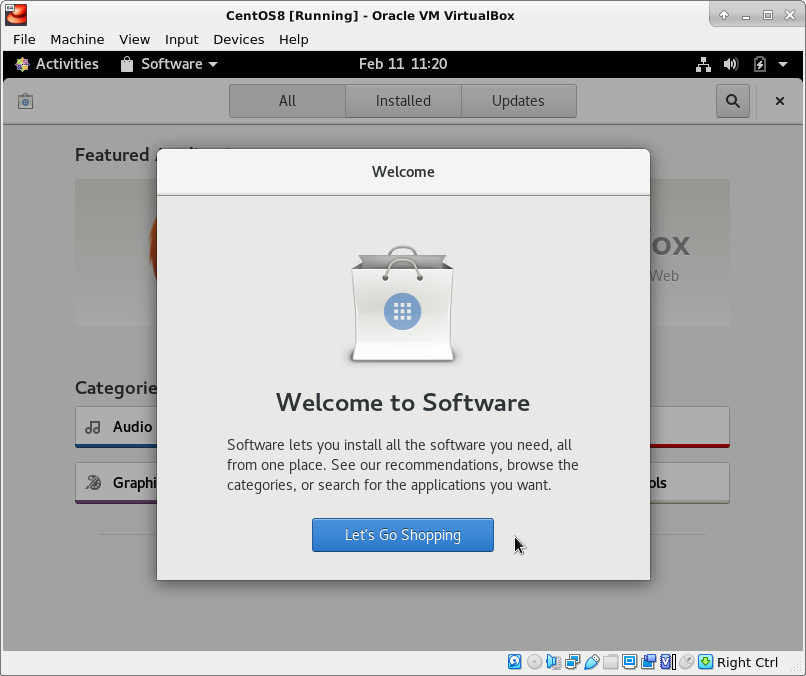
\includegraphics[width=0.9\textwidth]{linuxreader-img019.png}
	\caption{Software start scherm}
	\label{fig:de_software_start}
\end{figure}


